\chapter{Theoretische Grundlagen}
\label{cha:theogrund}

\section{Datenbankentwurf / ERM}
\label{sec:erm}

Unter dem Datenbankentwurf ist der Prozess zur Erstellung eines Schemas zu verstehen, welches die spätere Datenbank abbilden wird.
Hierunter fallen unter Anderem die Analyse der Anforderungen, aber auch die grafische Darstellung der Tabellen, in denen die Daten gespeichert werden.
Der Entwurf der Datenbank im vor der Implementierung ist essentiell, da im späteren Prozess Änderungen der Datenbankstruktur nicht nur die Datenbank selbst, sondern auch alle mit ihr verbundenen Applikationen betreffen werden.
Um die Beziehungen zwischen den einzelnen Tabellen korrekt darstellen zu können, wird das Entity-Relationship-Modell\footnote{vgl. Peter Pin-Shan Chen(1976): The Entity-Relationship Model--Toward a Unified View of Data. In: ACM Transactions on Database Systems, Vol 1, No 1, S.10} verwendet.
Durch dieses Modell lassen sich sogenannte ER-Diagramme zeichnen, z.B. nach der Chen Notation\footnote{vgl. Peter Pin-Shan Chen(1976): The Entity-Relationship Model--Toward a Unified View of Data. In: ACM Transactions on Database Systems, Vol 1, No 1, S.19}.
Ein ER-Diagramm nach Chen stellt die Entitätstypen (Klassen), Attribute, sowie Beziehungen (Relationen/Kardinalitäten) dar.
Im Folgenden Beispiel soll ein ER-Diagramm nach der Chen-Notation kurz erläutert werden.\\

Das nachfolgende Diagramm beschreibt Folgenden Sachverhalt:

\begin{itemize}
\item Ein Angestellter leitet mehrere Projekte.
\item Ein Projekt wird von einem Angestellten geleitet.
\end{itemize}

\begin{figure}[H]
\begin{center}
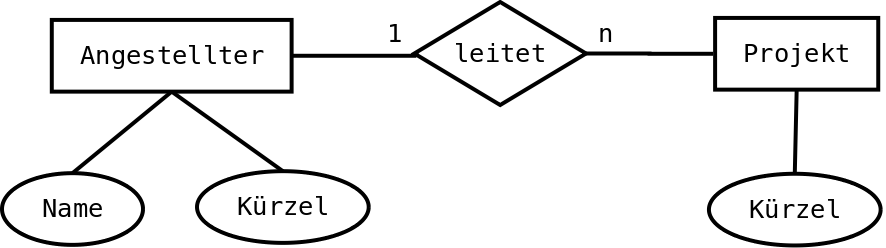
\includegraphics[scale=0.4]{img_chen_001.png}
\caption{Chen Notation 1:N}
\label{chenpic1}
\end{center}
\end{figure}

\begin{itemize}
\item Ein Autor verfasst mehrere Bücher.
\item Ein Buch wird von mehrere Autoren verfasst.
\end{itemize}

\begin{figure}[H]
\begin{center}
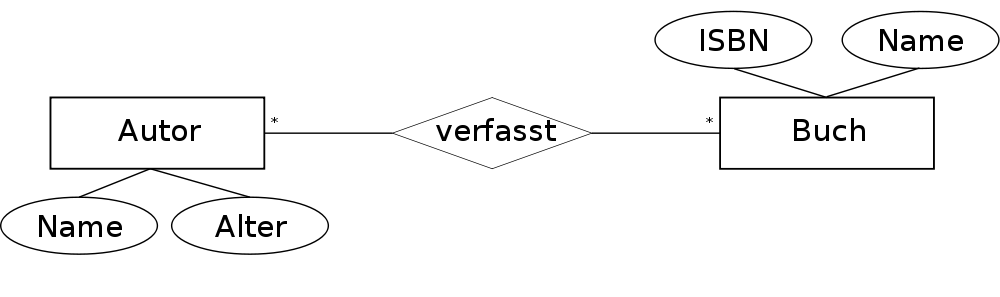
\includegraphics[scale=0.4]{img_chen_002.png}
\caption{Chen Notation N:M}
\label{chenpic2}
\end{center}
\end{figure}
\footnotetext{In Anlehnung an}

\section{Kardinalitäten}

Kardinalitäten beschreiben den Grad einer Verbindung zwischen zwei Objekten\footnote{vgl. Heinz Burnus(2007): Datenbankentwicklung in IT-Berufen, 1. Auflage, S.20}.
In Abbildung \ref{chenpic1} ist eine 1:n Kardinalität gegeben.
Diese sagt aus, dass einem Objekt der Relation 1, mehrere Objekte der Relation 2 zugeordnet werden, einem Objekt der Relation 2 jedoch nur ein Objekt der Relation 1.

In der zweiten Abbildung \ref{chenpic2} ist eine n:m Kardinalität zu sehen.
Diese sagt aus, dass einem Objekt der Relation 1, mehrere Objekte der Relation 2 angehören, einem Objekt der Relation 2 werden ebenfalls mehrere Objekten der Relation 1 zugewiesen.
Diese n:m Kardinalitäten müssen bei einem Datenbankentwurf aufgelöst werden, da hier keine eindeutige Zuordnung möglich ist. Meistens lässt sich eine solche Kardinalität wie in Abbildung \ref{chenpic2} durch das Hinzufügen einer zusätzliche Tabelle, welche beide Objekte verknüpft, lösen.
Ein Beispiel ist in Abbildung \ref{chenpic3} zu sehen.

\begin{figure}[H]
\begin{center}
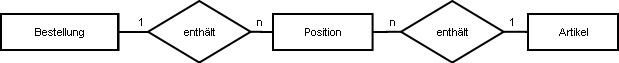
\includegraphics[scale=0.6]{chen_n_m_aufloesung.png}
\caption{Aufgelöste Chen N:M Notation}
\label{chenpic3}
\end{center}
\end{figure}

\section{Normalisierung - Optimierung von Datenbanken}
\label{secNormalisierung}
%\cite{codd1}
Wenn es bereits bestehende Datenbanken gibt, so muss geprüft werden, ob diese eine optimale Struktur aufweisen.
Eine Optimierung der Struktur ergibt sich nicht nur um eine bessere Übersichtlichkeit zu haben, sondern auch aus Gründen der Redundanz und der damit verbundenen Probleme.
Durch eine nicht benötige Redundanz kommt es zum Einen zu Geschwindigkeits und Platzverlusten innerhalb der Datenbank.
Da ein Wert an mehreren Stellen in der Datenbank steht kann es zu Problemen bei der Aktualisierung und Löschunge kommen, da alle Werte in der Datenbank geändert werden müssten und nicht nur ein Wert.
Dies kann anhand der sogenannten Normalisierung durchgeführt werden.\footnote{vgl. E. F. Codd(1970): A Relational Model of Data for Large Shared Data Banks in Commun. ACM, Vol 13, Nr. 6, S. 381} Dadurch lässt sich die Datenbank weiter optimieren.\footnote{vgl. Prof. Dr. Paul. Alpar(2001): Vorlesung, Datenorganisation und Datenbanken,  http://www.tekinci.de/skripte/DBDM/DB-SS2001.pdf}
Bei der Normalisierung wird abgefragt, ob Tabellen gewisse Eigenschaften erfüllen und sofern dies nicht der Fall ist, wird versucht diese zu erreichen.
Hierzu stehen bis zu 5 Stufen der Normalformen zur Verfügung.
Die 5 wichtigsten Normalformen beschreiben sich durch folgende Attribute.\footnote{vgl. Heinz Burnus(2007): Datenbankentwicklung in IT-Berufen, 1. Auflage, S.292-308}

\begin{enumerate}
\item Normalform: Alle Attribute besitzen einen atomaren Wertebereich
\item Normalform: Jedes Nichtschlüsselattribut ist vom kompletten Schlüssel abhängig
\item Normalform: Jedes Nichtschlüsselattribut ist von keinem Schlüsselkandidaten transitiv abhängig, dass heißt kein Attribut ist über ein anderes vom Hauptschlüssel abhängig
\item Normalform: Es darf in einer Relation nicht mehrere, voneinander unabhängige, 1:n-Beziehungen zu einem Schlüsselwert geben
\item Normalform: Es existieren nur noch Einzel-Abhänigkeiten
\end{enumerate}


In der ersten Normalform wird untersucht, ob jedes Attribut atomare Werte besitzt, dass heißt es enthält nur einen Wert und ist frei von Wiederholungen.\footnote{vgl. Matthias Schubert(2007): Datenbanken, Theorie, Entwurf und Programmierung relationaler Datenbanken, 2. Auflage, S.293}


\begin{figure}[H]
\begin{center}
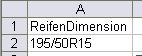
\includegraphics[scale=1]{img_chen_003.png}
\caption{Keine Normalform angewendet}
\label{chenpic4}
\end{center}
\end{figure}



In Abbildung \ref{chenpic4} ist eine Verletzung der Normalform 1. zu sehen. Um diese aufzuheben müssen wir die einzelnen Werte trennen wie in Abbildung \ref{chenpic5} zu sehen.

\begin{figure}[H]
\begin{center}
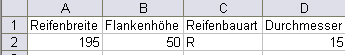
\includegraphics[scale=1]{img_chen_004.png}
\caption{1. Normalform}
\label{chenpic5}
\end{center}
\end{figure}

Wurde die Relation entsprechend angepasst, so ist Normalform 1 erreicht und es kann nun geprüft werden,
ob diese die Eigenschaften von Normalform 2 erfüllt.
Um eine Normalform zu erfüllen, müssen auch alle vorhergehenden Normalformen erfüllt sein, dass heißt erfüllt eine Tabelle die Normalform 3, so erfüllt sie auch die Normalform 1 und 2.


\section{Datenbankmanagementsysteme}
\label{sec:dbms}

Ein Datenbankmanagementsystem (DBMS) organisiert die Speicherung der Daten einer Datenbank und legt die Anordnung der Daten fest.
Das DBMS legt auch die Art der Beziehung fest, in der die Daten der Datenbank stehen (relational, objektorientiert).
Zur Kommunikation mit diesem wird eine Sprache benötigt. In diesem Zusammenhang wird die deskriptive Sprache SQL verwendet.\footnote{vgl. E. F. Codd(1970): A Relational Model of Data for Large Shared Data Banks in Commun. ACM, Vol 13, Nr. 6, S. 382}


Es gibt verschiedene Arten von DBMS:

\begin{itemize}
\item Hierarchisch
\item Relational
\item Objektorientiert
\end{itemize}

%BuchURL http://www.amazon.com/gp/product/354043187X
Ein hierarchisches DBMS\footnote{vgl. Bernd-Jürgen Falkowski(2002): Business Computing: Grundlagen und Standardsoftware, 1. Auflage, S.235} dient vor allem der schnellen Suche in großen Datenbanken.
Der Nachteil liegt darin, dass nur eine sequentielle Abarbeitung möglich ist und somit die Art der Abfragen mehr oder weniger schon im Voraus bestimmt sein muss.
Im Gegensatz hierzu stehen die relationalen Datenbanken, welche heutzutage den höchsten Verbreitungsrad besitzen.\footnote{Quelle}
Diese bieten eine flexible Auswertung der Daten durch die deklarative Abfragesprache SQL.
Es muss lediglich die Verknüpfung zwischen den Tabellen durch sogenannte JOINs hergestellt werden. Somit werden Primär- und Fremdschlüssel miteinander verknüpft.
Hinzu kommen die objektorientierten Datenbanken. Diese bieten die Möglichkeit Objekte von beliebiger Art und Weise ab zu speichern.
Problematisch hierbei sind jedoch die Formulierung von geeigneten Abfragen, weswegen diese in der Praxis eher selten und meist im Bereich von Multimedialen-Anwendungen anzutreffen sind.%\footnote{NOTIZ ODBMS evtl}

Wird versucht, verschiedene relationale DBMS in der Praxis zu vergleichen, so ist eine große Anzahl an verschiedenen Systemen zu finden.
Im Anschluss soll auf die, in der Praxis verwendeten, DBMS eingegangen werden.

\begin{itemize}
\item Microsoft Jet Engine (Access)
\item MS-SQL Server
\item Oracle
\item MySQL
\item PostgreSQL
\end{itemize}

Die Microsoft Jet Engine ist ein dateibasierendes DBMS, welches dem Benutzer eine einfache Möglichkeit bietet, Daten in einer Datenbank zu speichern und passende Oberflächen (Frontends) in der Datenbank zu integrieren.
Bei diesem System, wie bei allen anderen dateibasierenden DBMS, steht meist die einfache Konfigurierbarkeit im Vordergrund. Die Datenbanken sind meist für einen Einzeluser-Betrieb ausgelegt und spielen hier auch ihre Stärken aus.
Wird eine dateibasierende Datenbank von mehreren Usern benutzt so zeigen sich die Nachteile einer solchen Datenbank.
Dadurch, dass Access für jeden Nutzer bei einer Abfrage die komplette Datenbank durchsucht, entsteht eine hohe Auslastung der Festplatte, sowie des Netzwerks. Daher nimmt Geschwindigkeit bei mehreren Anwendern exponentiell ab, da sich alle Benutzer die Bandbreite der Festplatte sowie des Netzwerkes teilen.
Auch beim Speichern müssen zusätzlich Datensätze gesperrt und organisiert werden, da sonst die Daten inkonsistent werden können, wenn mehrere Personen gleichzeitig einen Datensatz schreiben.
MS-SQL ein relationales Datenbankmanagementsystem, welches ebenfalls von Microsoft erwerbbar
und in den verschiedenen Serverbetriebssystemen von Microsoft enthalten ist. Für Entwickler
ohne Enterpreise Lizenz wird eine eingeschränkte Express Version zur Verfügung gestellt. MS-SQL ist im Gegensatz zu Access kein dateibasierendes DBMS, sondern ein DBMS welches
zentral auf einem Server läuft. Hierdurch werden die Nachteile des dateibasierenden zu
den Vorteilen des serverbasierenden Systems. Da der Server selbst die Abfragen verwaltet
und zusätzlich Abfragen im Arbeitsspeicher ablegt, sowie dem Benutzer nur die Daten
sendet, die er auch angefordert hat und nicht die komplette Datei, werden Zugriffszeiten
und Netzwerk/Festplattenlast optimiert.\\
Ein weiteres DBMS stellt der Datenbankserver von Oracle dar. Die Lizenzstruktur ähnelt der von Microsoft, so gibt es auch hier kostenfreie und kostepflichtige Varianten. Im Gegenzug zum MS-SQL Server bietet Oracle ein breiteres Spektrum an Funktionalitäten und eine größere Konfigurationsmöglichkeit. Dieses wiederum macht sich im höheren Preis bemerkbar. Weitere Vorteile der Oracle Datenbank sind die weitgehende Betriebssystemunabhängigkeit, gute Dokumentation und der Support.

MySQL ist der Open Source Pendant zu MS-SQL, welches im Internet eine sehr hohen Verbreitungsgrad aufweist.
So wird dieses von Seiten wie Wikipedia\footnote{vgl. Mysql, http://www.mysql.com/why-mysql/scaleout/wikipedia.html} oder
Youtube\footnote{vgl. University of Maryland: How YouTube scales MySQL for its large databases, http://ebiquity.umbc.edu/blogger/2007/12/28/how-youtube-scales-mysql-for-its-large-databases/} verwendet.
Im Gegensatz zu MS-SQL erlaubt das GPL Lizenzmodell, dass die Datenbank für Privatanwender kostenlos ist und die Lizenzgebhren für Unternehmen einen Bruchteil der Kosten ausmachen, die für ein Microsoft System bezahlt werden müssten.\footnote{Vgl http://www.mindfactory.de/product\_info.php/pid/geizhals/info/p155132}

Eine weitere Datenbank stellt PostgreSQL dar, welches unter der BSD-Lizenz zur Verfügung gestellt wird und somit auch für kommerzielle Projekte ohne Kosten nutzbar ist\footnote{vgl. PostgreSQL: BSD-Lizenz, http://www.postgresql.org/about/licence}.


\section{Webserver}
\label{sec:websrv}

Ein Webserver dient zum Bereitstellen von statischen, sowie dynamischen HTML Seiten.
Der Vorteil bei Webservern liegt darin, dass nur Informationen ausgetauscht werden, die der Nutzer auch angefordert hat.
Weiterhin bietet es den Vorteil, diese zielgerichteten Informationen einer größeren Menge an Benutzern zur Verfügung zu stellen, ohne dass spezielle Vorkehrungen zur späteren Skalierung getroffen werden mssen.

Um dynamische Webseiten erzeugen zu können, bedarf es einer Skriptsprache.
Aktuell haben sich folgende Sprachen etabliert:\footnote{vgl. Tiobe Software(2009): TIOBE Programming Community Index for August 2009, http://www.tiobe.com/index.php/content/paperinfo/tpci/index.html}

\begin{itemize}
\item ASP - Active Server Pages
\item JSP - JavaServer Pages
\item PHP - PHP: Hypertext Preprocessor
\end{itemize}

ASP ist eine Skriptsprache der Firma Microsoft und basiert grundlegend auf der Syntax von Visual Basic.
JSP dient dem selben Zweck, wurde jedoch von Sun entwickelt und besitzt die Syntax von Java.
PHP ist eine Skriptsprache, welche sich hauptsächlich an der C Syntax orientiert und speziell für das Erstellen von
dynamischen Webseiten erstellt wurde. Sie ist die am weitesten verbreitete Scriptsprache zum Erstellen von dynamischen Webseiten.

Da alle der aufgeführten Skriptsprachen weitgehend Webserver-/Plattformunabhängig sind, kann man frei zwischen den meist benutzten Webserverprogrammen wählen, hierunter fallen unter Anderem:


\begin{itemize}
\item Apache
\item IIS - Internet Information Services
\end{itemize}

Der Apache Webserver ist ein Opensource Webserver der Apache Foundation.
Er kann unter vielen verschiedenen Betriebssystemen eingesetzt werden und unterstützt durch seine Module alle verbreiteten Scriptsprachen, sowie Datenbanken.

Der IIS Webserver von Microsoft läuft ausschließlich unter Windows, zudem ist es auch nur unter dem Serverbetriebssystem von Windows möglich mehr als 10 Verbindungen gleichzeitig aufzubauen.\footnote{vgl. Microsoft: IIS 7.0: Übersicht über die verfügbaren Features in IIS 7.0, http://msdn.microsoft.com/de-de/library/cc753198\%28WS.10\%29.aspx}

\section{Schnittstellen}
\label{sec:schnittstellen}


Um eine Verbindung zwischen den einzelnen Komponenten herzustellen, wird eine passende API benötigt.
Idealerweise bringt jedes DBMS und jeder Webserver passende Treiber mit, obwohl dieser Fall nicht immer gegeben ist.

Zur Zeit haben sich verschiedene Varianten etabliert:

\begin{itemize}
\item Native Treiber
\item ODBC (Open Database Connectivity)
\item JDBC (Java Database Connectivity)
\item ADO (ActiveX Data Objects)
\end{itemize}

Jedes etablierte DBMS bietet für Entwickler eine native Schnittstelle zum Ansprechen der Datenbank an.
Diese wird meist in verschiedenen Programmiersprachen angeboten, unter Anderem C/C++, PHP usw. .
Die native Methode besitzt den Vorteil, dass sie das Nutzen aller Funktionen der Datenbank ermöglichen, wohingegen dafür keine einheitlichen Design Patterns existieren, was die Verwendungen von mehreren
verschiedenen DBMS erschwert.

Aufgrund dessen hat sich in der Vergangenheit unter Windows die sogenannte Open Database Connectivity-Schnittstelle (ODBC) etabliert, welche es ermöglicht ohne Veränderung des Quellcodes das Datenbanksystem zu wechsel.
Hierzu muss lediglich der ODBC-Eintrag angepasst werden. Ein weiterer Vorteil, der sich durch die Schnittstelle ergibt, ist die Möglichkeit alle Abfragen im standardisierten SQL absetzen zu können, unabhängig vom vewendeten DBMS.
Neben der ODBC-Schnittstelle gibt es auch das JDBC System bei Java. Zwar kann Java auch die ODBC-Schnittstelle über eine Treiber-Brücke nutzen, aber laut Oracle \footnote{Vgl. Oracle: JDBC-ODBC Bridge Driver, http://download.oracle.com/javase/1.3/docs/guide/jdbc/getstart/bridge.doc.html} soll dies nur im experimentellen Gebrauch stattfinden.
Da der Einsatz eines nativen JDBC Treibers verhindert, dass unerwünschten Zustände auftreten, welche z.B. bei einer JDBC-ODBC Anbindung möglich sind, ist die Verwendeung des nativen Treibers vorzuziehen.
Zusätzlich gibt es noch ADO von Microsoft, welches auch als Schnittstelle für Webserver mit IIS bzw. ASP dient.
Diese ähnelt in der Verwendung JDBC, da ebenfalls ein ODBC-Treiber angesteuert werden kann.
Der Verbindungsaufbau ist ähnlich einfach gestaltet und ermöglicht auch für Webanwendungen eine einfache Anbindung an die Datenbank.

\section{Softwareentwicklung}
\label{sec:softdev}

Unter der Softwarentwicklung ist die Herstellung und Entwicklung von Software, sowie die dazugehörige Planung und Modellierung dieser zu verstehen. Die Softwareentwicklung umfasst eine Vielzahl von Teilgebieten. Die Entwicklung einer komplexen Software wird anhand eines strukturierten Projektplans vorgenommen, welcher den Entwicklungsprozess inhaltlich und zeitlich abgrenzt. Die Software wird anhand von bestimmten Schritten fertiggestellt, welche miteinander eng verzahnt sind. Unterschieden wird bei der Softwarentwicklung zwischen Individualsoftware und Standardsoftware. Bei der Standard-Software handelt es sich um Software, welche einen klar definierten Anwendungsbereich abdeckt und als vorgefertigtes Produkt erworben werden kann. Standardsoftware zeichnet sich somit aus, dass diese über mehrere Kunden hinweg ohne Anpassung einsetzbar ist. Ein Beispiel hierfür sind branchenunabhängige Software, wie z.B. das Office-Paket, aber auch Branchensoftware, welche zielgerichtet für eine Branche ist und in dieser übergreifend eingesetzt werden kann.\\
Bei der Individualsoftware handelt es sich um Software, welche individuell für einen Kunden angefertigt wurde. Typisch für Individualsoftware ist es, dass zuvor keine passenden Lösungen an Standardsoftware existiert haben.  Es kann aber auch sein, dass die Entwicklung einer Indivdualsoftware trotz existierender Standardsoftware Sinn macht, sofern es monitär vortelhaft ist.
Ein weiterer Punkt  könnte der Versuch einen Wettbewerbsvorteil gegenüber den Wettbewerbern zu erhalten oder die Optimierung einer vorhandenen Lösung sein.\\
Die Umsetzung eines Projektes findet entweder intern oder von einem externen Dienstleister statt. Eine wichtige Rolle spielen ebenfalls die Vorgehensweisen bei der Umsetzung eines Projektes. Hier gibt es die Wahl zwischen stark strukturierten Herangehensweisen, wie das Wasserfallmodell bis hin zu sehr flexiblen, z.B. der Agilen Softwareentwicklung.\\
Im Folgenden soll auf die wichtigsten Kernprozesse bei der Umsetzung eines Systems in einem Projekt eingegangen werden.\\
\\
Planung\\
\\
Zu Beginn einer Systementwicklung steht die Planung. In dieser werden die Anforderungen erhoben. Hierbei handelt es sich um das Sammeln aller Anforderungen die seitens des Kundens oder aufgrund von externen Einflüssen (z.B. Gesetze) gegeben sind. Währenddessen ist vor allem der Dialog mit dem Kunden, aber auch mit den späteren Benutzern sowie den fachlichen Experten notwendig. In dieser Phase wird neben dem Lastenheft (Anforderungsdefinition) auch das Pflichtenheft erstellt. Es erfolgt auch eine Aufwandseinschätzung, sowie die Wahl des Vorgehensmodells.\\
\\
\\
Analyse\\
\\
Im Analyse-Prozess findet die Auswertung der zuvor gesammelten Anforderungen statt. Bei dieser Auswertung kommt es auch zur Analyse der Prozesse und des Systems. Bei der Systemanalyse kommt es bereits zum ersten Modellentwurf, wobei dieser explizit ohne “Maschinen” d.h. ohne systemspezifische Inhalte ist und somit technische Details noch nicht ins Modell aufgenommen werden. Sofern die Möglichkeit besteht wird in diesem Prozess auch ein Mock-up erstellt. Bei einem Mock-up handelt es sich um ein Modell bzw. einer Nachbildung welches meist eine Attrappe darstellt. In der Softwareentwicklung wird darunter ein Prototyp verstanden, welcher rudimentär die Benutzerschnittstelle widerspiegelt. Er wird vor allem zu Beginn des Projektes eingesetzt um eine bessere Zusammenarbeit mit dem Auftraggeber und dem späteren Anwender zu erlangen. Somit können die Anforderungen an die Benutzeroberfläche direkt besprochen werden und die Beteiligten sich ein besseres Bild über die spätere Anwendung machen.\\
\\
\\
Entwurf\\
\\
Beim Entwurfsprozess geht es um die Planung der Software-Lösung. Zur Planung von dieser werden unterschiedliche Sprachen zur Modellierung verwendet. Die wichtigste Sprache hierbei ist UML, welche unter Anderem auch die Modellierung von Klassen und Objekten, sowie deren Beziehungen untereinander ermöglicht. Auf UML wird in Kapitel X detailliert eingegangen.
Zum Entwurf gehören ebenfalls System- bzw. Designentscheidungen, die später in die Programmierung einfließen.
\\
\\
Programmierung\\
\\
Bei der Programmierung geht es letztendlich um die Umsetzung des zuvor entworfenen Systems. Hierbei wird je nach Vorgehensweise die strukturierte oder objektorientierte Programmierung angewandt.
\\
\\
Validierung und Verifizierung
\\
Bei der Validierung  und Verifizierung geht es vor allem um Tests. Hierbei wird unterschieden zwischen Low-Level-Tests und High-Level-Tests. Unter Low-Level-Tests sind solche Test zu verstehen, die während der Implementierung an Teilen des Systems stattfinden. Bei High-Level-Tests wird das komplette System getestet. Einer der Low-Level-Tests ist der Modultest. Bei diesem werden einzelne Module im Programm getestet.  Diese Tests werden regelmäßig während der Entwicklung durchgeführt. Ein weiterer Low-Level-Test ist der Integrationstest. Bei diesem werden verschiedene Module in Kombination getestet. Für jede Verbindung zwischen zwei Komponentne wird ein Test erstellt, welcher überprüft, ob diese ordnungsgemäß nach der Spezifikation funktionieren. In kleinereren Projekten findet der Integrationstest meist während der Implementierung durch die Programmierer statt.
Der so genannte Systemtest ist ein High-Level-Test bei dem das gesamte Programm gegen die zuvor definierten Anforderungen gegen geprüft wird. Dieser Systemtest findet meist in einer Testumgebung statt und erhält meist simulierte Testdaten um die bestehende Produktivumgebung nicht weiter zu beeinträchtigen. Die simulierten Testdaten können trotz Allem den reellen Daten entsprechen, sollen jedoch verhindern, dass das System direkt in die Produktivumgebung einwirkt.
Der letzte High-Level-Test dient der Abnahme und wird auch als Akzeptanztest bezeichnet. Bei diesem Test geht es um den Test der Software im produktiven Einsatz beim Kunden. Der Test selbst stellt ein Black-Box-Test dar und dient meist zu Rechnungsstellung bzw. Abnahme in Verbindung mit den Testprotokollen.

\section{Unified Modeling Language}
\label{sec:uml}

Die Unified Modeling Language (UML) ist eine standardisierte graphische Modellierungssprache im Bereich der Softwareentwicklung. Der Standard wird von der Object Management Group verwaltet und wurde auch von dieser geschaffen. UML enthält verschiedene Notationstechniken um visuelle Modelle von softwareintensiven System zu erzeugen. UML selbst ist auch von der ISO standardisiert und zählt heutzutage zu einer der bedeutesten Modellierungssprachen bei der Softwareentwicklung. Durch die Sprache wird nicht nur eine grafische Notation festgehalten sondern ebenfalls die Begriffe und die jeweiligen Beziehungen zwischen diesen. Somit bilden die Diagramme nur eine Teil dessen ab, was unter der UML zu verstehen ist.
Die UML wird seit 1997 weiterentwickelt und ist seitdem in mehrere Versionen erschienen.
Die in der UML verwendeten Modelle lassen sich in verschiedene Kategorien unterteilen, die wie folgt lauten:\\
\\
-Struktur-Diagramme\\
-Verhaltens-Diagramme\\
\\
In diese Kategorien lassen sich wiederum die in UML verwendeten Diagramme einordnen:\\
-Strukturdiagramme\\
    * Klassendiagramm\\
    * Kompositionsstrukturdiagramm\\
    * Komponentendiagramm\\
    * Verteilungsdiagramm\\
    * Objektdiagramm\\
    * Paketdiagramm\\
    * Profildiagramm\\
-Verhaltensdiagramme\\
    * Aktivitätsdiagramm\\
    * Anwendungsfalldiagramm\\
    * Interaktionsübersichtsdiagramm\\
    * Kommunikationsdiagramm\\
    * Sequenzdiagramm\\
    * Zeitverlaufsdiagramm\\
    * Zustandsdiagramm\\
\\
Im Folgenden soll nun auf die wichtigsten Diagramme eingegangen werden, welche für die Umsetzung des Projekts selbst verwendet wurden.\\
Das erste verwendete Diagramm, ist das Anwendungsfalldiagramm (im
folgenden als Usecase-Diagramm benannt).  Dieses dient dazu einen Überblick über die Funktionen des Systems, aber auch über die beteiligten Personen (Akteure) zu erhalten. Das Usecase-Diagramm stellt keine Beschreibung der Abläufe dar, sondern die Beziehung zwischen Akteur und den jeweiligen Funktionen, die in diesem Fall als Anwendungsfall bezeichnet werden. Akteure können im Diagramm Anwender, Administratoren, aber auch Systeme selbst darstellen, welche von extern auf das System zugreifen. Im Diagramm selbst werden diese als 'Strichmännchen' dargestellt und haben jeweils einen Namen. In einem Usecase-Diagramm muss immer mindestens ein Akteur vorhanden sein.
Anwendungsfälle hingegen werden als Ellipsen dargestellt und enthalten eine Beschreibung.
Um beide unterschiedliche Elemente in einer Gruppe zusammenzufassen, wird ein Rahmen um alle beteiligten Elemente gebildet.
Dieser wird im Systemkontext genannt und bilder somit die Systemgrenze.
Neben den normalen Assoziationen (z.B. Benutzer -> Drucken) besteht die Möglichkeit der Generalisierung.
Das bedeutet, dass zwei spezifische Akteure oder Anwendungsfälle zu einem generellen zusammengefasst werden können.
Ein Beispiel eines Usecase-Diagramms ist in Abbildung X zu sehen.\\
\\
\begin{figure}[H]
\centering
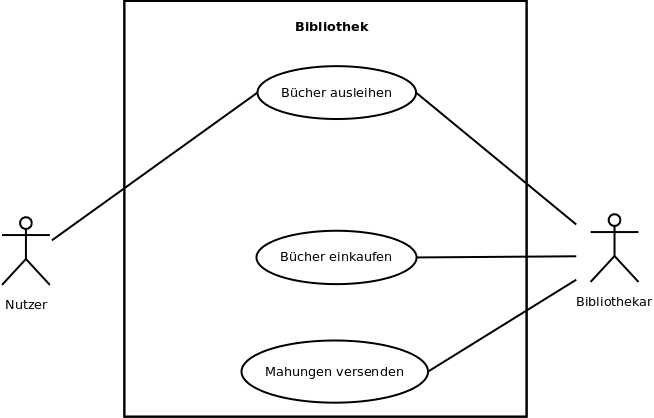
\includegraphics[width=0.7\textwidth]{uml_usecase_ex.png}
\caption{Usecase-Diagramm}
\label{fig:show_s1_s2_p1_n1}
\end{figure}
Ein weiteres wichtiges Diagramm stellt das Klassendiagramm dar. Es dient zur Beschreibung einzelner Klassen sowie deren Beziehungen untereinander. Klassen dienen zur Beschreibung der Objekte, welche von diesen instanziert werden. Im Klassendiagramm wird eine Klasse als Rechteck dargestellt und neben dem Klassenamen enthält diese ein Bereich für die Attribute, sowie für die Methoden.
Um die Sichtbarkeit der Attribute und Methoden darzustellen, werden verschiedene Symbole verwendet:\\

     + für public, unbeschränkter Zugriff\\
     \# für protected, Zugriff nur von der Klasse sowie von Unterklassen (geerbte Klassen)\\
     \- für private, nur innerhlab der Klasse selbst sichtbar\\
     \~ für package, innerhalb des Pakets sichtbar\\
\\
Ähnlich wie bei einem Usecase-Diagramm bietet sich beim Klassendiagramm die Möglichkeit einer Generalisierung.
Beispielsweise sind die Klassen \textit{PKW} und \textit{LKW} Unterklassen von der Klasse \textit{Fahrzeuge}. In Abbildung X ist ein Beispiel eines Klassendiagramms zu sehen.\\
\\
\begin{figure}[H]
\centering
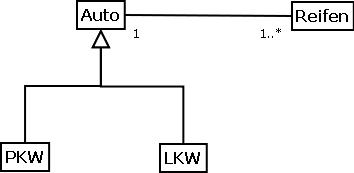
\includegraphics[width=0.7\textwidth]{uml_class.png}
\caption{Klassendiagramm}
\label{fig:show_s1_s2_p1_n1}
\end{figure}
Ebenfalls relevant für die Umsetzung des Projektes sind die Aktivitätsdiagramme.
Sie dienen dazu, Abläufe von Prozessen abzubilden.
Beim Aktivitätsdiagramm befinden sich die Elemente in abgerundeten Rechtecken, welche zusätzlich den Namen der Aktivität neben den Elementen enthalten.
Den Start bzw. Endpunkt bilden jeweils ein gefüllter Kreis, wobei der Endpunkt nur teilweise gefüllt ist. Aktivitäten werden in abgerundeten Rechtecken aufgelistet und miteinander in Flussrichtung verbunden. Entscheidungsfälle werden durch eine Raute symbolisiert.
Je nach Entscheidungsfall verläuft der Pfad bei ‘Ja’ weiter in Flussrichtung nach unten, oder bei einer Abweichung zur Seite ab.
Zusätzlich bietet sich die Möglichkeit, Aktivitäten parallel ablaufen zu lassen.
Dies kann durch Aktivitäten, die zwischen zwei Balken liegen, symbolisiert werden.
Im Folgenden ist in Abbildung X ein beispielhaftes Aktivitätsdiagramm zu sehen.\\
\\
\begin{figure}[H]
\centering
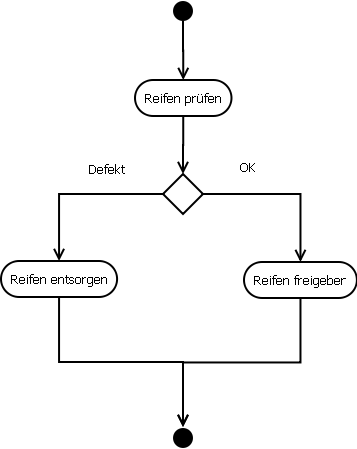
\includegraphics[width=0.7\textwidth]{uml_activity.png}
\caption{Aktivitätsdiagramm}
\label{fig:show_s1_s2_p1_n1}
\end{figure}
Für das bessere Verständnis der späteren Implementierung ist das Sequenzdiagramm ebenfalls von größerer Bedeutung. Es dient dazu, einen Überblick über die Lebensdauer und Interaktion zwischen den einzelnen Klassen bzw. deren Objekte zu erhalten.
Bei diesen wird nicht nur auf die bei den Klassendiagrammen gezeigte Beziehung, sondern auch auf den Nachrichtenaustausch zwischen den Objekten eingegangen.
Bei einem Nachrichtenaufruf mit Antwort bzw. mit einer daraus folgenden Aktion, wird es notwendig zu unterscheiden, welche Art von Kommunikation stattfindet. Hierbei gibt es die synchrone, als auch asynchrone Kommunikation.
Bei der synchronen Kommunikation handelt es sich um ein Nachrichtenaustausch bei der das aufrufende Element, beispielsweise ein Browser der Daten anfordert (eine Webseite), wartet, bis die Daten empfangen wurden. Hierbei sendet er die Anfrage für die jeweilige Seite ab und muss anschließend warten bis der Server ihm diese zurückgeliefert hat. Erst im Anschluss kann der Browser die Webseite dem Nutzer darstellen.
Bei der asynchronen Kommunikation handelt es sich um einen Austausch, welcher es nicht erfordert, dass ein Teilnehmer auf die Bestätigung des Anderen warten muss. Beispielsweise beim Versand einer Email. Hier muss der Sender weder warten bis der Empfänger online ist, noch muss er den Empfang der Email abwarten. Hier können Nachrichten gesendet werden, ohne dass für den Sender ein Ergebnis zur Laufzeit erwartet wird.
Eine Nachricht wird im Sequenzdiagramm durch Pfeile dargestellt. Synchrone Nachrichten werden mit gefüllten Pfeilspitzen, asynchrone Nachrichten mit offenen Pfeilspitzen gekennzeichnet. In der Nachfolgenden Abbildung ist ein beispielhaftes Sequenzdiagramm zu sehen.\\
\\
\begin{figure}[H]
\centering
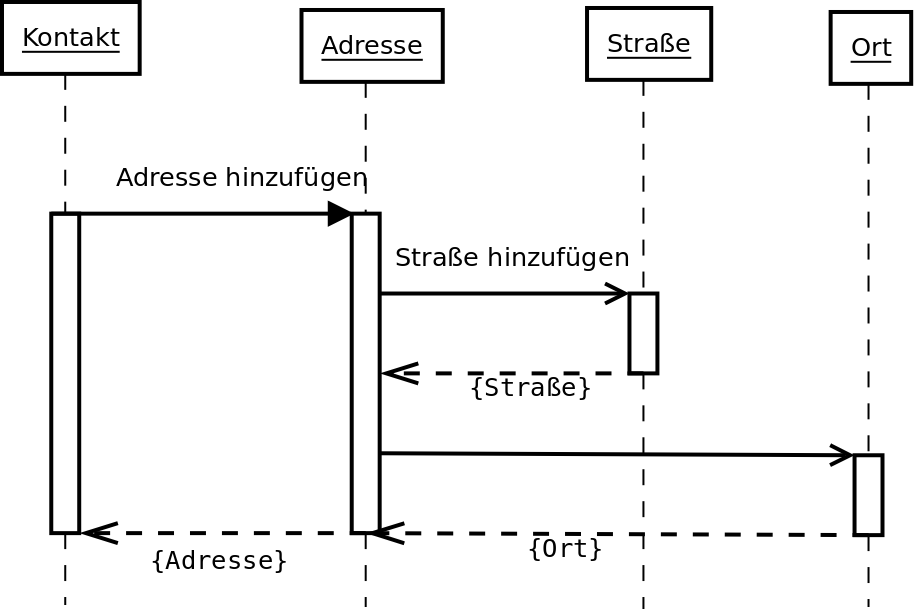
\includegraphics[width=0.7\textwidth]{uml_seq.png}
\caption{Sequenzdiagramm}
\label{fig:show_s1_s2_p1_n1}
\end{figure}

\section{Media Access Control}
\label{sec:mac}

Bei der MAC-Adresse (Media-Access-Controll-Adresse) handelt es sich um eine Adresse eines Netzwerkadapters, die zur eindeutigen Identifizierung in einem Netzwerk dient. MAC-Adressen werden in einer Vielzahl von Netzwerk Protokollen verwendet.
Unter Anderem wird sie im Ethernet-Protokoll (IEEE 802.3), aber auch vielen anderen Netzwerktechnologien genutzt die unter den IEEE 802 Gruppen zu finden sind.
Das MAC-Protokoll steuert die Adressierung auf Hardwareebene, sowie die Zugriffsart.
Im ISO/OSI-Modell ist das MAC-Protokoll auf Schicht 2, der Sicherungsschicht, angesiedelt.
Somit hat das MAC-Protokoll zwei Aufgaben. Zum Einen die Adressierung eines Gerätes und zum Anderen wie dieses Gerät auf das Medium zugreift.\\
Zur eindeutigen Adressierung der Netzwerkadapter  dient die sogenannte MAC-Adresse. Hierbei handelt es sich um einen 48-bit Wert, der einzigartig auf der ganzen Welt sein sollte.\footnote{vgl. ...} Durch die Änderbarkeit der MAC-Adresse kann es jedoch vorkommen, dass dies nicht immer gegeben ist. Die Wahrscheinlichkeit eine doppelte MAC-Adresse im Netzwerk zu haben ist jedoch extrem gering, da der Adressraum nach aktuellen Kalkulationen noch bis in das Jahr 2100 ausreicht.\footnote{http://standards.ieee.org/develop/regauth/tut/eui.pdf} Die ersten 24-bit kennzeichnen den Hersteller des Netzwerkadapters, die anschließenden 24-bit sind beliebig vom Hersteller vergebbar.
Einige bestimmte MAC-Adressen können jedoch nicht reserviert werden, da es sich hierbei handelt um Broadcast-Adressen und Multicast-Adressen handelt.
Eine MAC-Adresse kann wie folgt dargestellt werden:\\
\\
01-23-45-67-89-ab oder 01:23:45:67:89:ab oder 0123.4567.89ab\\
\\
Anhand der Herstellerkennung lassen sich wiederum Rückschlüsse auf das Netzwerkgerät ziehen.
Die Hersteller, welche sich jeweils hinter der Herstellerkennung verbergen, sind öffentlich bei der IEEE einsehbar, z.B. per Internet.\footnote{http://standards.ieee.org/develop/regauth/oui/public.html}\\
Das MAC-Protokoll regelt ebenfalls den Zugriff auf das Transportmedium. Hierbei wird in zwei verschiedene Zugriffsarten unterteilt. Zum Einen den kontrollierten Zugriff und zum Anderen der konkurrierende Zugriff.
Beim kontrollierten Zugriff wird darauf geachtet, dass keine Kollision auftritt. Somit kommuniziert keines der Netzwerkgeräte gleichzeitig über einen Kanal, sondern es ist immer nur ein Gerät aktiv.\\
Beim konkurrierenden Zugriff hingegen darf jedes Gerät auf das Medium zugreifen, jedoch gibt es bestimmte Regeln, wenn eine Kollision auftritt. In diesen wird geregelt in welcher Art und Weise die Kollisionen behandelt werden. In der Praxis gibt es unter Anderem das Protokoll CSMA/CD.
Dieses stellt bei einer Kollision durch ein Stör-Signal sicher, dass alle beteiligten Geräte die Kollision ebenfalls erkennen.
Zusätzlich versendet das Gerät das Paket nach einer Zeit wiederum erneut, bis dieses ankommt oder die Anzahl der maximalen Versuche überschritten wurde. Die Wartezeit steigt exponentiell anhand der Versuche.
Hierzu wird eine Zufallszahl aus dem Bereich 0 und (2\^i)-1 ms gewählt.
Wobei i für den i-ten Versuch steht.

\section{Virtual Local Area Network}
\label{sec:vlan}

Bei einem VLAN (Virtual Local Area Network) handelt es sich um ein logisches Netzwerk innerhalb eines physikalischen Netzwerkes.
Dieses logische Netz beinhaltet meist nur einen gewissen Teil des physikalischen Netzwerkes.
VLANs können über einen oder mehrere Switches ausgedehnt werden und müssen sich nicht auf einen speziellen Port beziehen.
Um ein Netzwerk durch VLANs in mehrere Teilnetze zu unterteilen gibt es den Ansatz Ports bzw. die einzelnen Datenpakete jeweils VLANs zuzuweisen.
Durch diese Zuweisung findet eine logische Trennung statt, da nur die Geräte in einem VLAN untereinander kommunizieren können.
Die Unterteilung des bestehenden Netzwerkes in Teilnetze bewerkestelligt VLAN dadurch, dass es Switches, die VLAN unterstützen, dazu veranlasst, Frames (Datenpakete) eines VLANs nicht in ein anderes VLAN weiterzuleiten, auch wenn beide physikalisch an den selben Switch angeschlossen sind.
VLANs können über verschiedene Arten realisiert werden.
VLANs lassen sich in portbasierte VLANs und tagged VLANs unterschieden.

Bei den portbasierten VLANs gehört ein Port je einem VLAN an oder ist ein Trunk-Port.
Bei einem Trunk-Port handelt es sich um ein Port über den mehrere VLANs geschaltet sind.\\

Das sogenannte tagged VLAN hingegen findet im Unterschied zu den portbasierten VLANs die Kennzeichnung im Ethernet-Frame selbst statt.
Dieses 'tagging' ist nach IEEE 802.1q spezifiziert.\footnote{Vgl. IEEE 802.1q}
Beim tagged VLAN kennzeichnen die Switches am Einspeiseort oder spezielle tagging-fähige Geräte die Pakete.
Diese Pakete werden wiederum von den Switches am Endgerät detagged oder wiederum von tagging-fähigen Gerät selbst.\\
Zusätzlich gibt es eine Unterscheidung zwischen statischen und dynamischen VLANs.
Bei einem statischen VLAN ist ein Port einer speziellen VLAN-Art zugeordnet.
Entweder zu einem Port-basierten VLAN oder zu einem tagged VLAN, wobei ein Port mehreren VLANs angehören kann und dieser dann ein Trunk-Port ist.\\
Das dynamische VLAN hingegen ist nicht portbasierend und richtet sich nach dem Inhalt des Frames. Jedoch ist zu beachten, dass die Inhalte eines Frames beliebig veränderbar sind und somit dynamische VLANs nicht in sicherheitskritischen Netzwerken verwendet werden sollten.
Die Zugehörigkeit zu einem VLAN kann per Adresse (MAC oder IP), auf Basis des Protokolls (IP, AppleTalk, IPX) oder auch auf Anwendungsebene nach Portnummern (80,443).
So ist es möglich, z.B. ein mobiles Endgerät im Netzwerk immer dem gleichen VLAN zuordnen zu lassen, unabhängig an welchem Ort dieses angeschlossen ist.\\

Die Gründe für die Verwendung eines VLANs lassen sich in drei Punkte aufteilen.
Zuerst macht eine Verwendung wie oben bereits erwähnt Sinn, wenn eine flexible Zuordnung eines Endgerätes immer zum selben VLAN gemacht werden muss.\\
Ein weitere Grund für VLANs sind Performance-Aspekte. Neben der Priorisierung von speziellen Daten (z.B. VOIP), dient ein VLAN meist der Verkleinerung der Broadcast-Domänen.
Durch die Verkleinerung der Domänen, wird ein Broadcast nicht über das gesamte Netzwerk hinweg geschickt.\\
Neben diesen Aspekten spielt die Sicherheit ebenfalls eine wichtige Rolle.
Um zu verhindern, dass das Netzwerk abgehört wird, kann es sinnvoll sein, VLANs einzusetzen.
Der Grund hierfür liegt darin, dass VLANs gegenüber Layer-2-Attacken architekturbedingt unempflindlich sind.


\section{SNMP}
\label{sec:snmp}
Unter dem Simple Network Management Protocol ist ein Netzwerkprotokoll zu verstehen, welches einem erlaubt Netzwerkgeräte (z.B. Drucker, Router, Switches, Router) per Netzwerk zu überwachen und zu steuern.\footnote{vgl. Essential SNMP, S. 1}
Diese Abfragen werden von einem zentralen Punkt aus durchgeführt, dem sogenannten SNMP-Manager, welcher die Daten von den SNMP-Agenten (Netzwerkelementen) abruft.\footnote{vgl. Essential SNMP, S. 3}\\
Bei SNMP handelt es sich um ein Protokoll, welches sich auf der Schicht 7, die Anwendungs-Ebene, des ISO/OSI-Schichtenmodells, ansiedeln lässt.
Entwickelt wurde das Protokoll von der IEFT und ist über diverse RFCs definiert.
Durch die hohe Modularität ist SNMP unabhängig von IP und funktioniert somit auch über IPX oder AppleTalk. Dies ist mitunter auch ein Grund für die weite Verbreitung von SNMP, welches mittlerweile als Standard gilt.\\
Die Funktionsweise von  SNMP spiegelt sich in der Verwendung der Agenten und Manager wieder.
Zunächst gibt es die sogenannten Agenten welche als Dienst auf dem jeweiligen Endgerät laufen und die Informationen zur Verfügung stellen. Diese werden dann auf einem Manager jeweils abgerufen per SNMP. Die Nachrichten werden entweder angefordert vom Manager oder aufgrund eines Ereignisses vom Agent an den Manager selbständig gesendet.\\
SNMP selbst definiert nicht welche Daten/Werte die Netzwerkkomponenten liefern, sondern gibt nur eine Baumstruktur vor, an die sogenannte Management Information Base (MIB) angliedert.
Diese beschreibt die jeweils enthaltenen Informationen und sind teilweise ebenfalls über RFCs spezifiziert.\footnote{vgl. RFC 1213} Zusätzlich gibt es herstellerspezifische MIBs z.b. von Cisco , die in einem speziellen Punkt im Baum hinterlegt werden können. Diese MIBs werden unter dem  Object Identifier (OID) 1.3.6.1.4.1 (iso.org.dod.internet.private.enterprises) bei der IANA registriert.\\
Bei der Kommunikation untereinander werden verschiedene Paket-Typen verwendet.

GET\\

Bei den GET Paketen handelt es sich um jeweils unterschiedliche Arten der Anforderung die vom Manager an den Agent gesendet werden.\\
Bei einem normalen GET-Paket wird ein einzelnes Attribut vom Agenten angefordert. Jedoch gibt es Abfragen, bei denen nicht im Voraus bekannt ist, wie viele Attribute abgefragt werden müssen. Beispielsweise der Status mehrerer Ports an einem Switch. Da dem SNMP-Manager jedoch keine Informationen vorliegen wie viele Ports der Switch hat, kann er nicht im Voraus die entsprechende Abfrage starten.\\

GETNEXT\\

Um diese Problematik zu lösen gibt es den sogenannten GETNEXT-Befehl, der es ermöglicht den Wert sowie die OID eines daraufolgenden Elementes zu erhalten.\\
//<Beispiel>\\

Die Abfrage von x Ports erzeugt x+1 Abfragen (Bei einem 48 Port Switch somit 49 Abfragen) ist ineffektiv , da der Manager nur eine Informationsmenge erhalten möchte aber dazu eine Vielzahl an Anfragen durchführen muss.

GETBULK\\
Daher wurde mit SNMP v2 der GETBULK Befehl eingeführt. Dieser ermöglicht es mehrere Werte mit einer Abfrage zu erhalten, die am Knoten im Baum hinterlegt sind.\\

SET\\
Das SET-Paket dient zum setzten spezieller Werte, so kann zum Beispiel darüber der Status des Ports von einem Switch  geändert werden, oder es könnte eine Firewall konfiguriert werden.

RESPONSE\\
Auf diese bisher genannten Pakete antwortet der Agent mit einem RESPONSE Paket, welcher die benötigten Werte oder eine Fehlermeldung enthält.
Sofern beim SNMP-Agent z.B. gewisse Grenzwerte hinterlegt wurden kann dieser sich bei einer Überschreitung mittels eines Trap-Paketes beim Manager melden, ohne das dieser die Information explizit abgefragt hat.\\
Um möglichst wenig Netzwerklast zu erzeugen kommuniziert SNMP über das UDP Protokoll, da es eine verbindunglose Kommunikation ermöglicht. Der Agent erhält die Anfragen auf Port 161, während der Manager auf Port 162 die Trap Meldungen empfängt.\\
TRAP\\





\section{Cisco Discovery Protokoll}
\label{sec:cdp}

Das Cisco Discovery Protokoll (CDP) von Cisco ist ein proprietäres Protokoll, welches dazu dient, Cisco-Geräten zu ermöglichen andere angeschlossene Geräte zu identifizieren und mit diesen Informationen auszutauschen. Es kann allerdings auch zum sogenannten “On-Demand-Routing” verwendet werden. Hierbei handelt es sich um eine cisco-spezifische Erweiterung von CDP, welche es ermöglicht ein simples Routing zu erstellen.
Die Cisco Geräte senden jeweils zur Multicast-Adresse “01-00-0c-cc-cc-cc”, welche auch von anderen Cisco-Protokollen (Z.B. VTP) verwendet wird. Dies geschieht in einem Intervall von 60 Sekunden auf allen relevanten Interfaces. Jedes der Beteiligten Cisco Geräte führt intern eine Tabelle mit den Informationen über die Geräte, welche in der “Nachbarschaft” gefunden wurden. Hierunter fallen Dinge wie IP, Alias, Geräte-Typ und auch Informationen über die dort befindliche Software bzw. das Betriebssystem.
Bei einem Cisco-Swicth wird zum Beispiel nicht nur die Beschreibung (IOS) sondern auch Modell, IOS-Version, Link-Status (Geschwindigkeit, Duplex) und viele weitere Informationen ausgelesen.
Diese können per internen Befehl oder per SNMP abgefragt werden. Bei jedem Empfang von CDP Daten, werden die internen Tabellen gepflegt und die Haltbarkeitszeit wieder zurückgesetzt, da Geräte die sich nicht mehr melden nach einer bestimmten Zeit (Standardmäßig nach 180 Sekunden) aus den Tabellen wiederum entfernt werden. Die Informationen welche übertragen werden sind einfach erweiterbar, da diese auf dem “Type-Length-Value” Format basieren. Das heißt in einer Nachricht wird zuerst der Typ des Attributs bestimmt (Z.b. String, Zahl, Datum) danach die Zeichenlänge des Wertes und der Wert selbst.\\
Hersteller wie HP, distanzieren sich zunehmend von diesem proprietären Protokoll und unterstützen das durch die IEEE spezifizierte offene Protokoll LLDP, welches Hersteller unabhängig ist und den selben Funktionsumfang beinhaltet.